
The data format of WINTERC 5.4 is quite complicated and is best summarised as follows:

\begin{center}
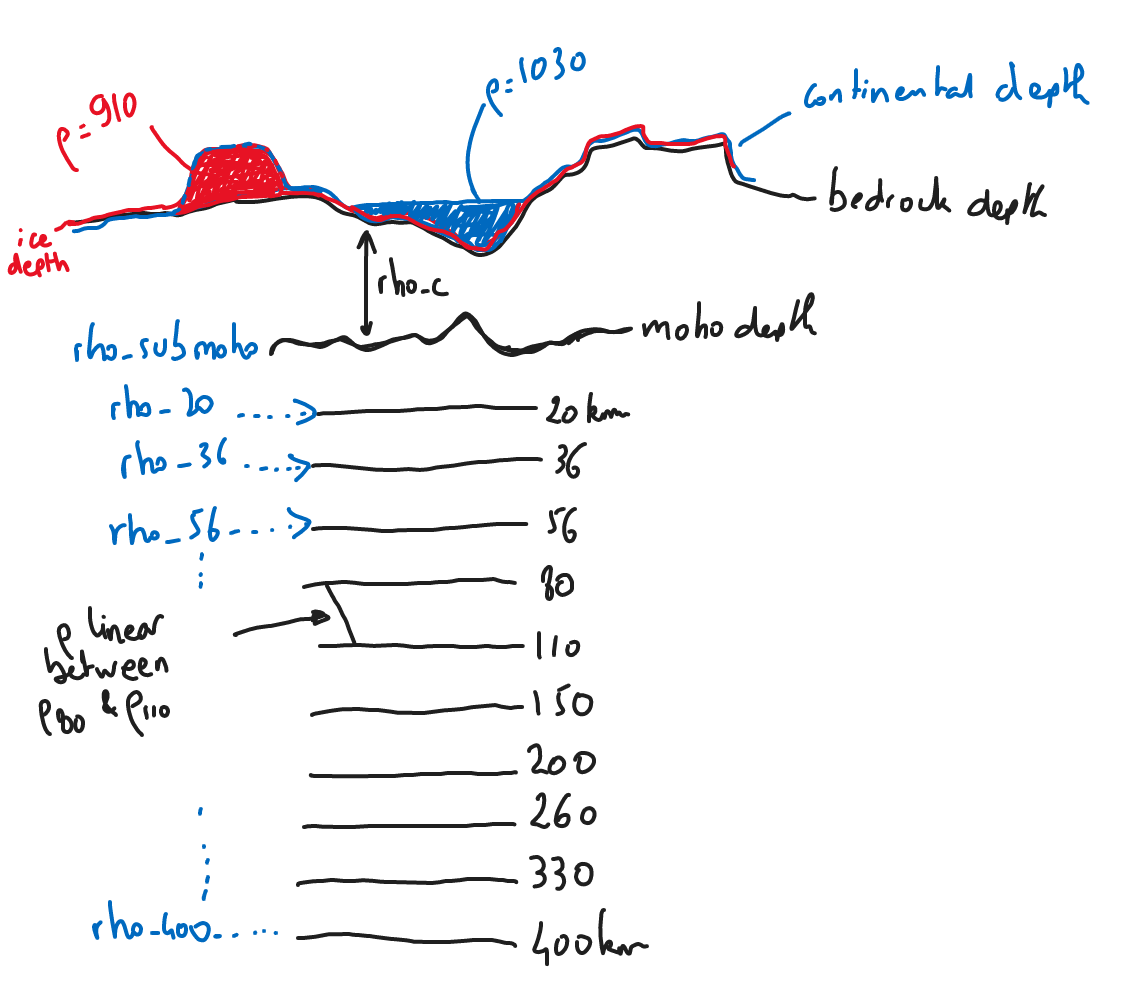
\includegraphics[width=9cm]{python_codes/fieldstone_99/images/whiteboard}
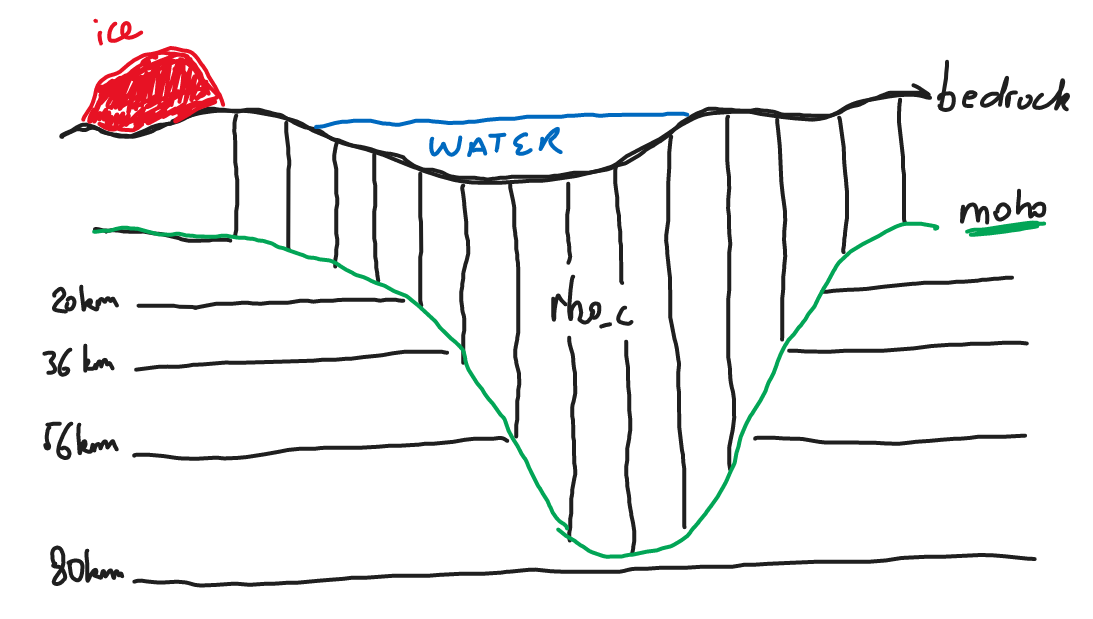
\includegraphics[width=6cm]{python_codes/fieldstone_99/images/whiteboard2}
\end{center}

Below 20km depth densities are given at various depths (36, 56, 80, 110, 150, 200, 260, 330 and 400km)
and values in between should be interpolated linearly. 
There are four files
{\asciifile ETOPO2\_km\_continental.xyz}, 
{\asciifile ETOPO2\_km\_depth\_Bed.xyz}, 
{\asciifile ETOPO2\_km\_depth\_Ice.xyz} and 
{\asciifile Global\_Moho\_CRUST1.0.xyz}
which contain the location of these four boundaries at 1/4 degree resolution. 


\begin{center}
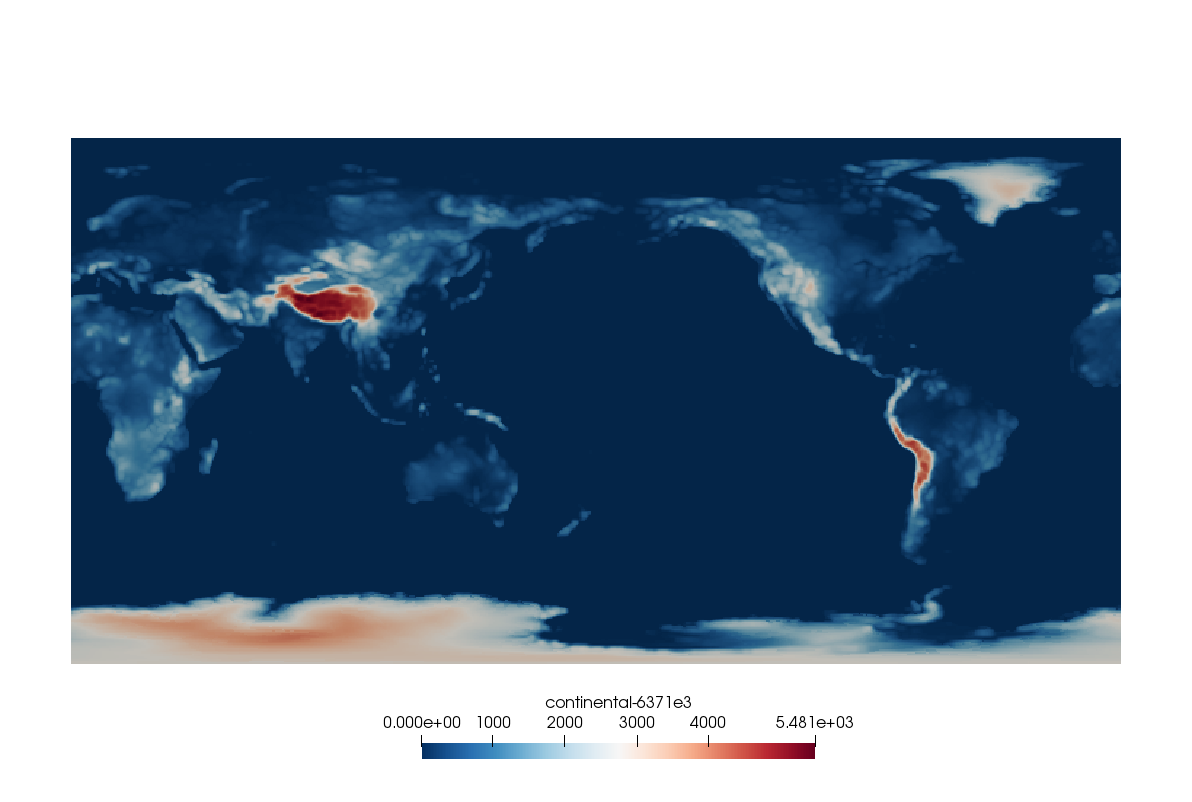
\includegraphics[width=8cm]{python_codes/fieldstone_99/images/continental}
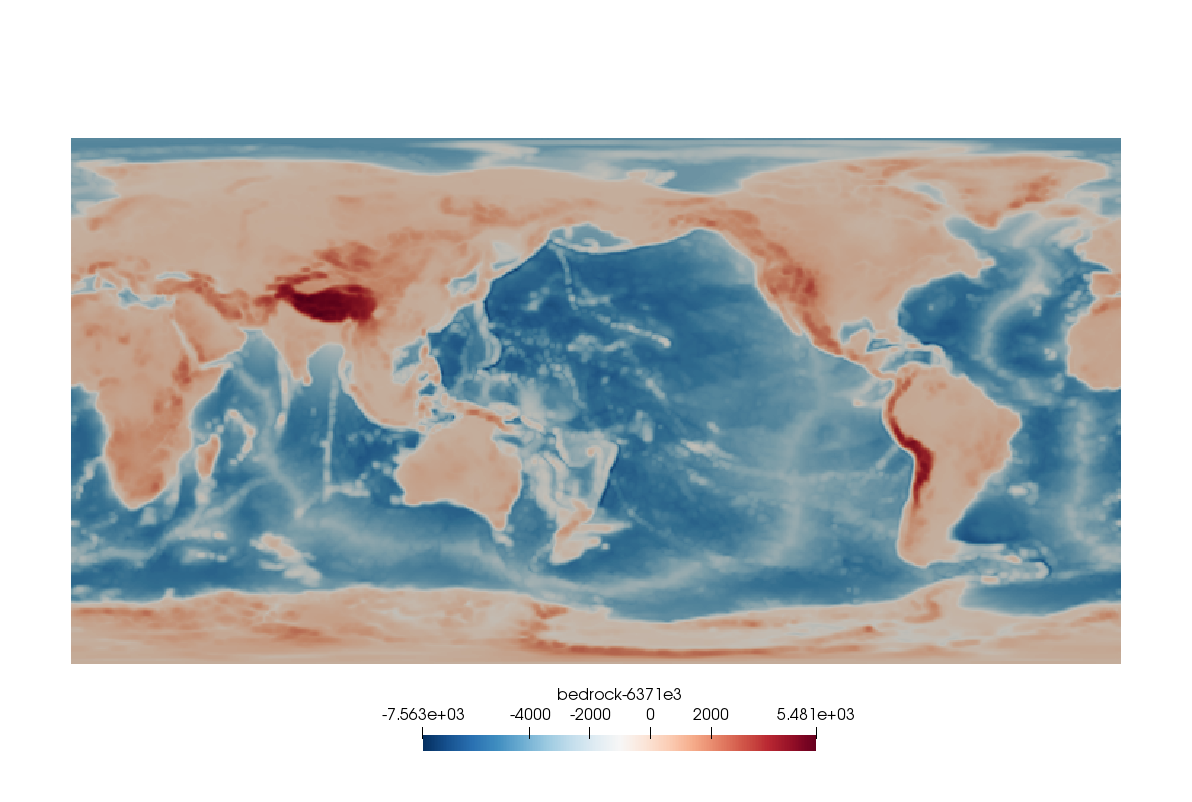
\includegraphics[width=8cm]{python_codes/fieldstone_99/images/bedrock}\\
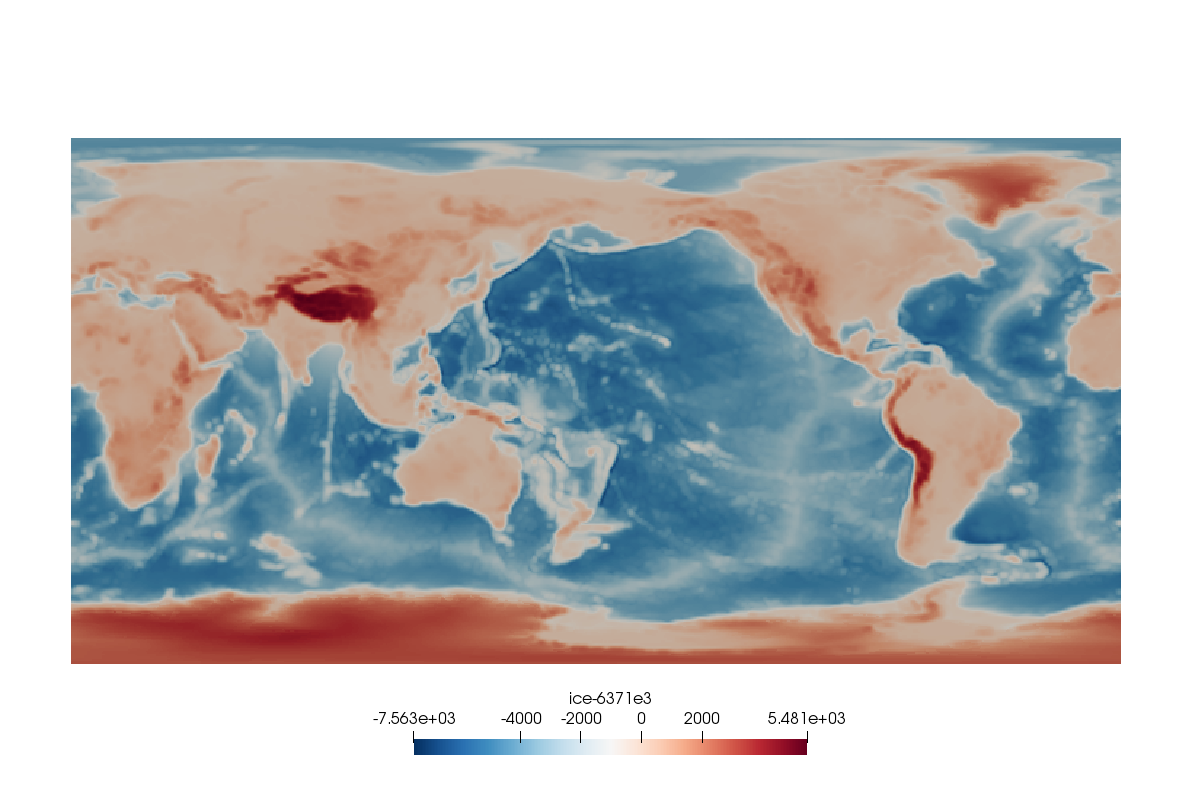
\includegraphics[width=8cm]{python_codes/fieldstone_99/images/ice}
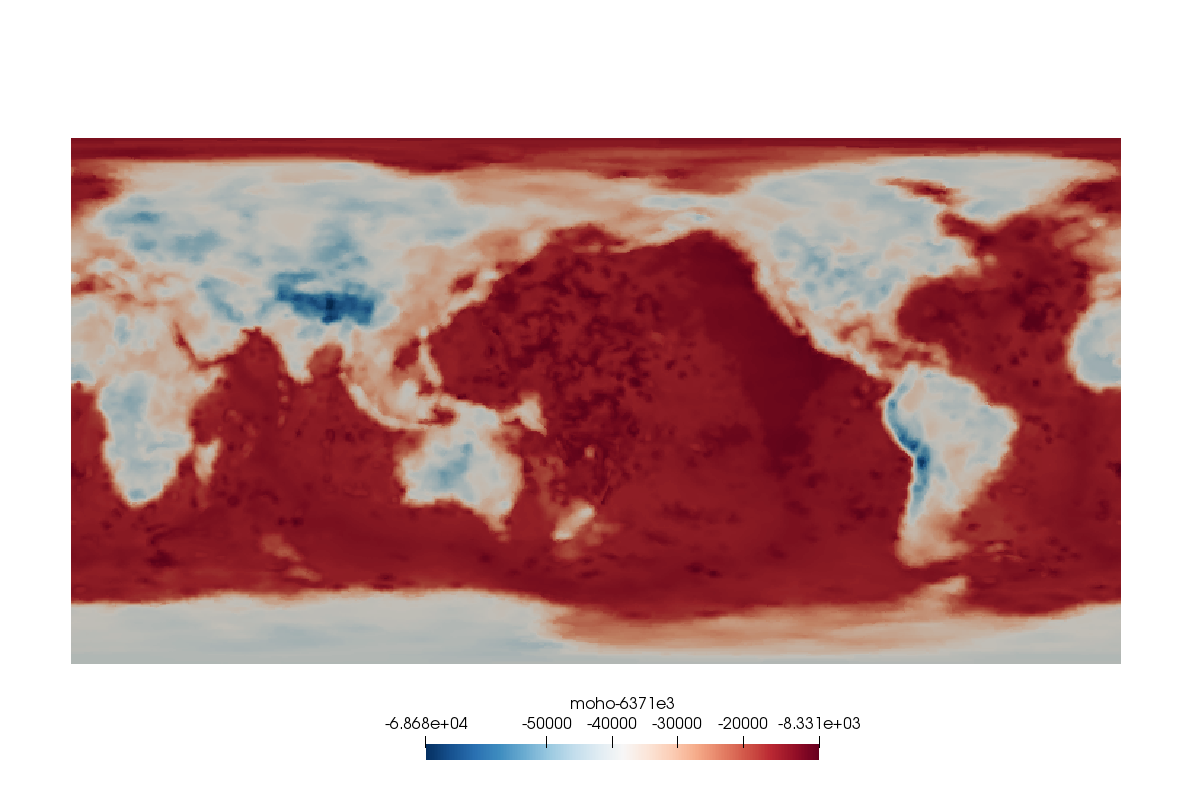
\includegraphics[width=8cm]{python_codes/fieldstone_99/images/moho}\\
{\captionfont Topography of the four key layers.}
\end{center}

\begin{center}
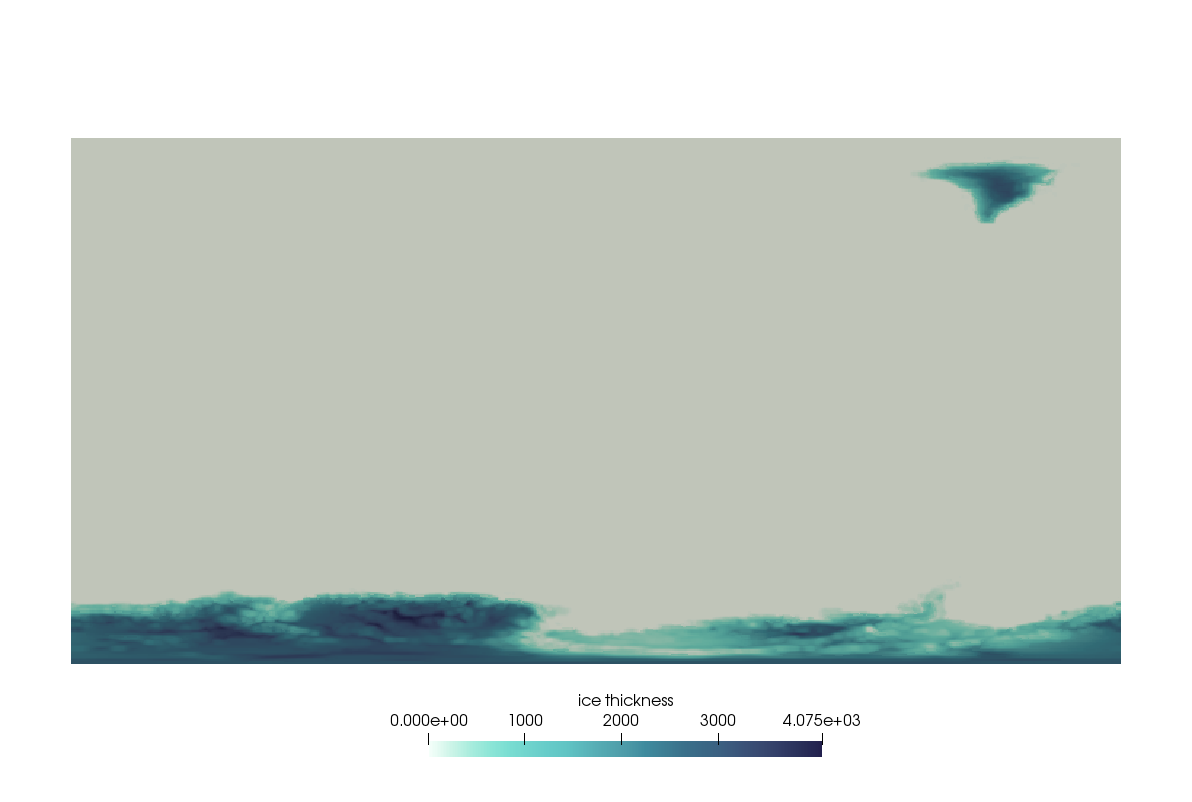
\includegraphics[width=8cm]{python_codes/fieldstone_99/images/ice_thickness}
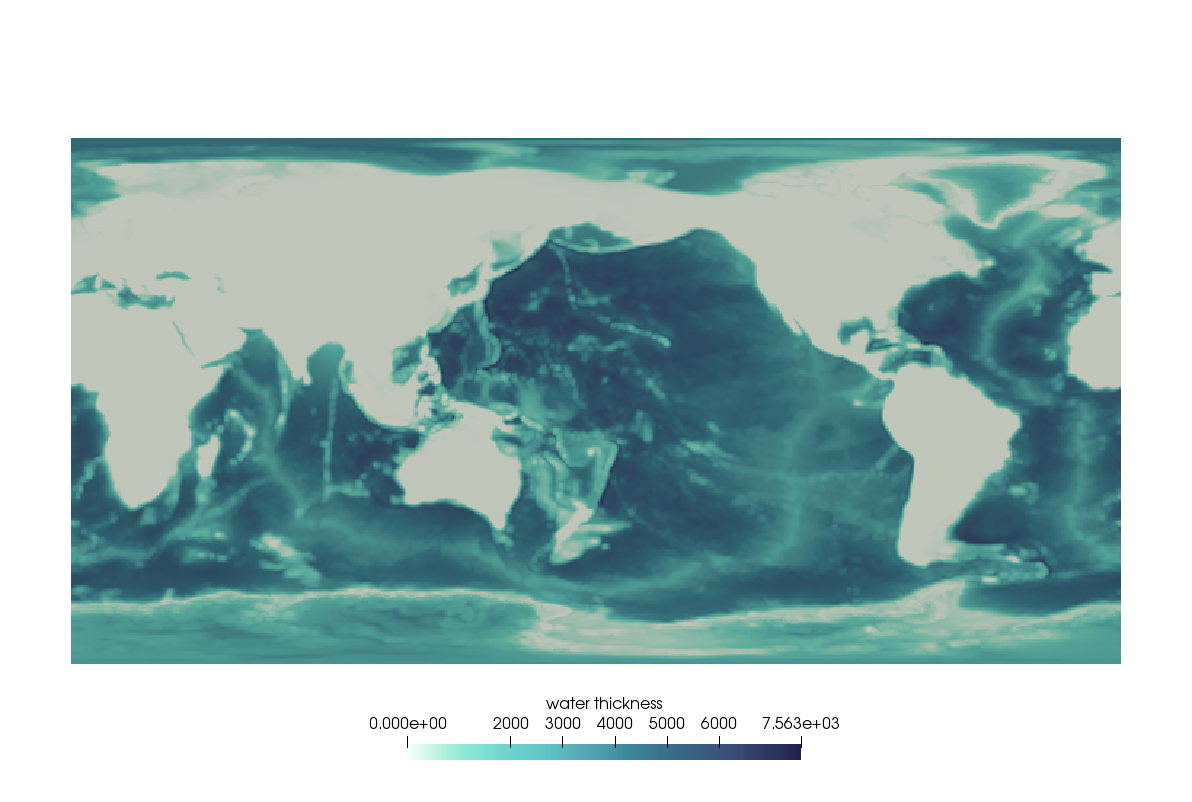
\includegraphics[width=8cm]{python_codes/fieldstone_99/images/water_thickness}\\
{\captionfont computed thicknesses of ice and water.}
\end{center}

Between the bedrock and the moho the density is radially constant but changes 
laterally. It is stored in {\asciifile rho\_c\_out.xyz}.
The moho has its own density file {\asciifile rho\_submoho\_out.xyz}
Water has a density of 1030\si{\kg\per\cubic\metre} and ice of 910\si{\kg\per\cubic\metre}.

\begin{center}
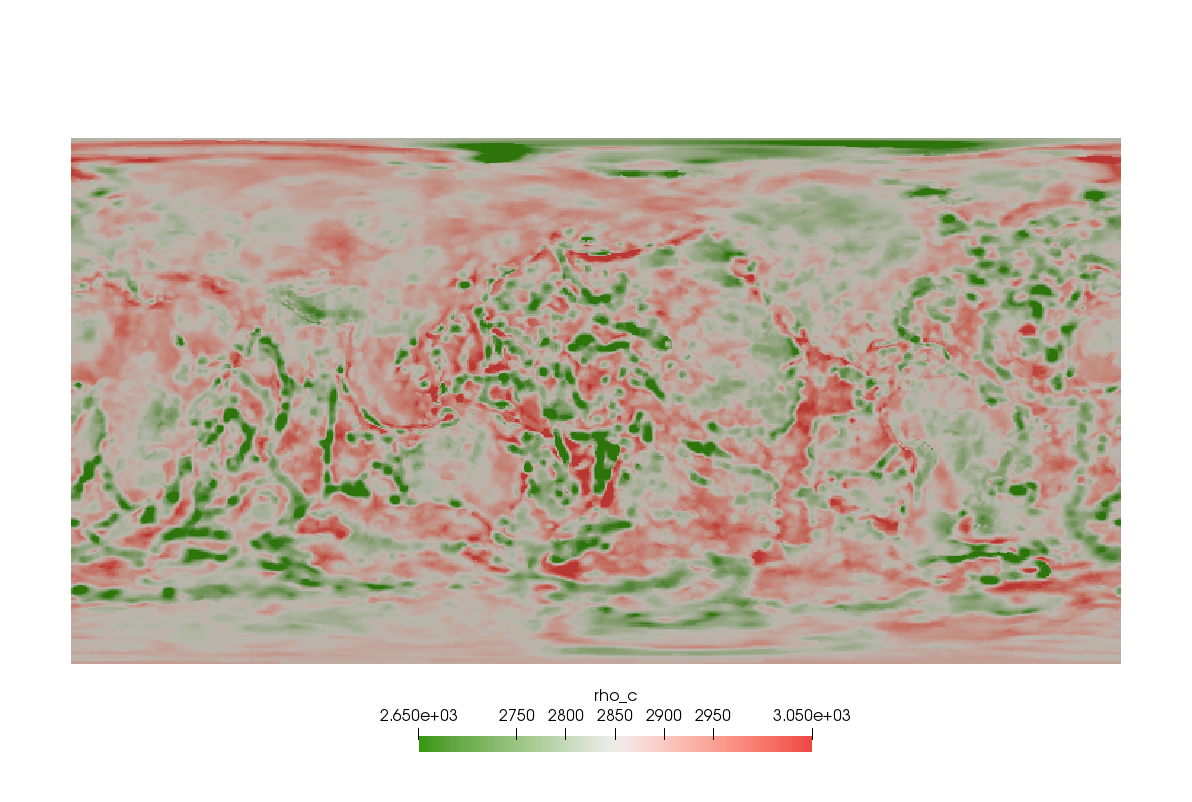
\includegraphics[width=8cm]{python_codes/fieldstone_99/images/rho_c}
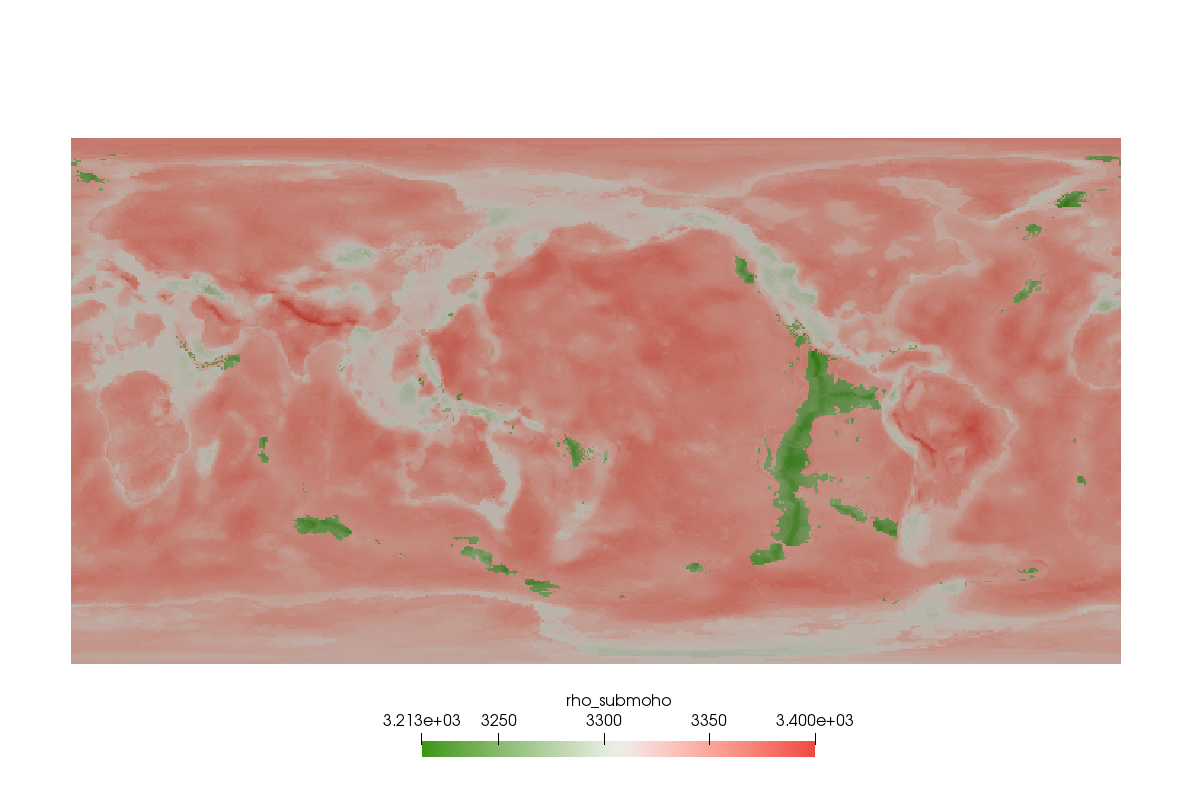
\includegraphics[width=8cm]{python_codes/fieldstone_99/images/rho_submoho}\\
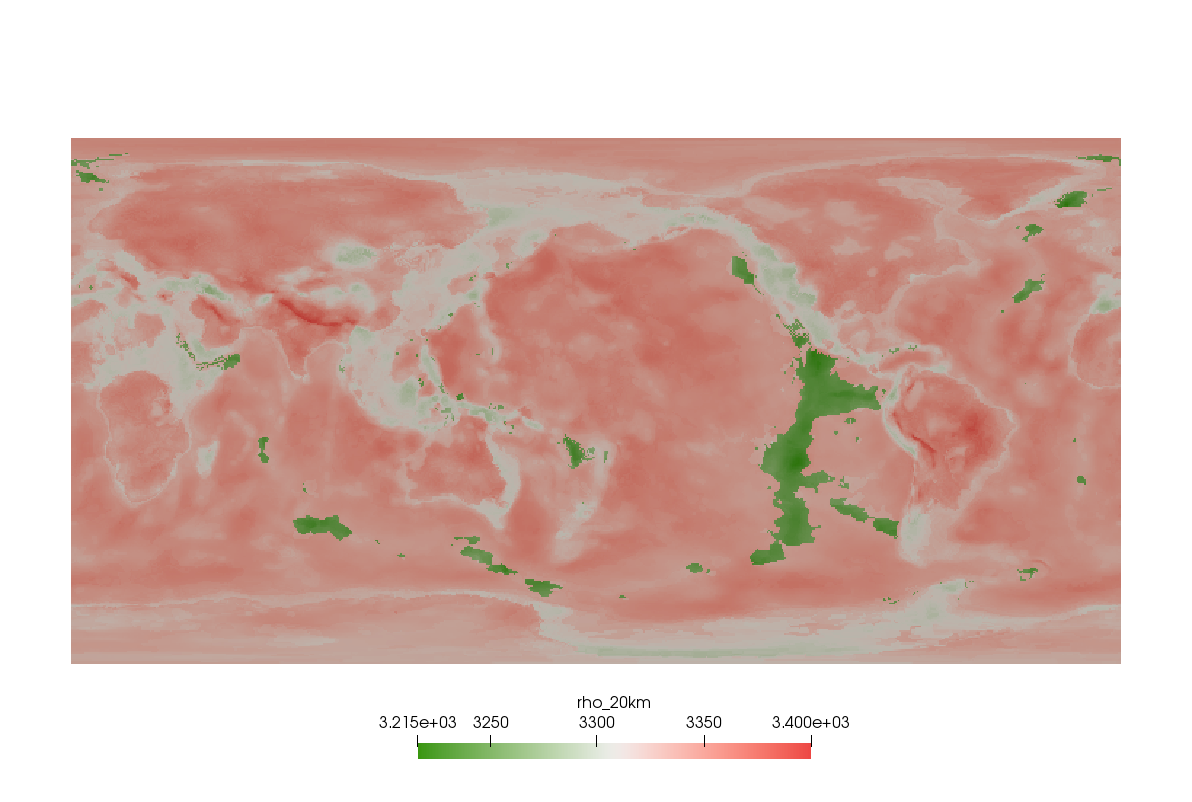
\includegraphics[width=8cm]{python_codes/fieldstone_99/images/rho_20}
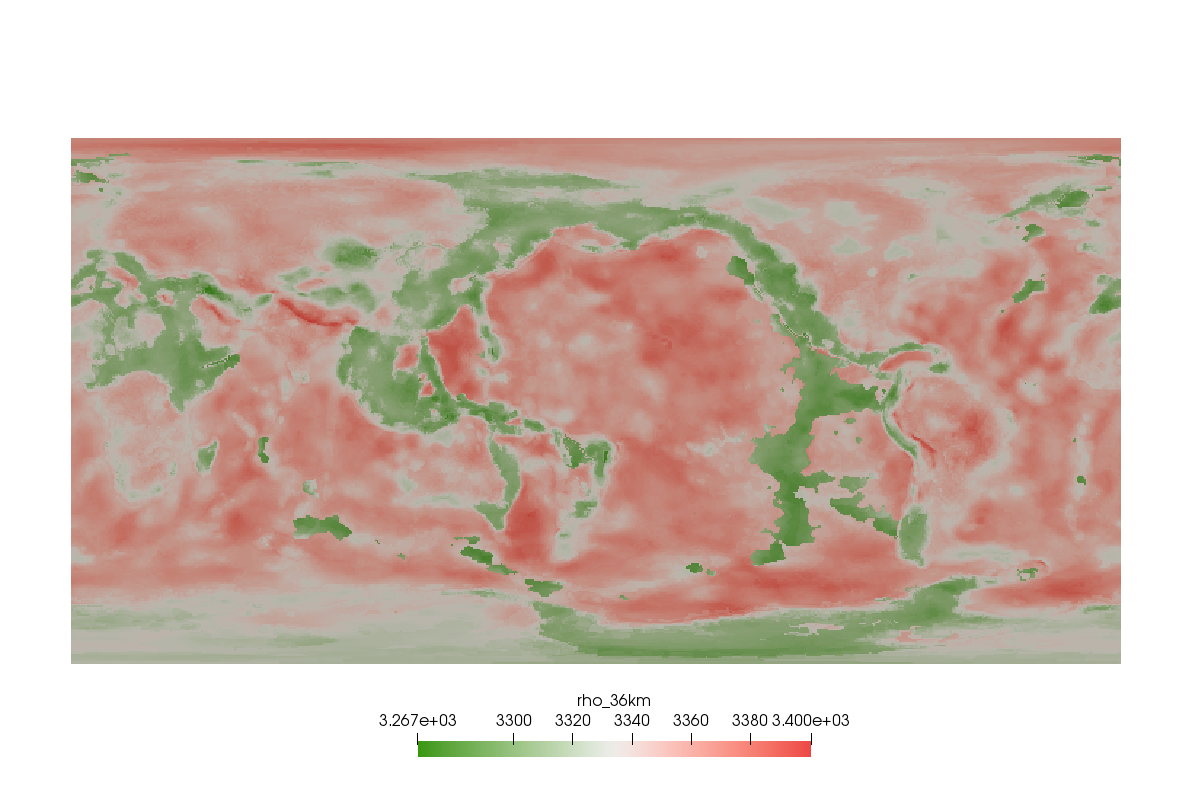
\includegraphics[width=8cm]{python_codes/fieldstone_99/images/rho_36}\\
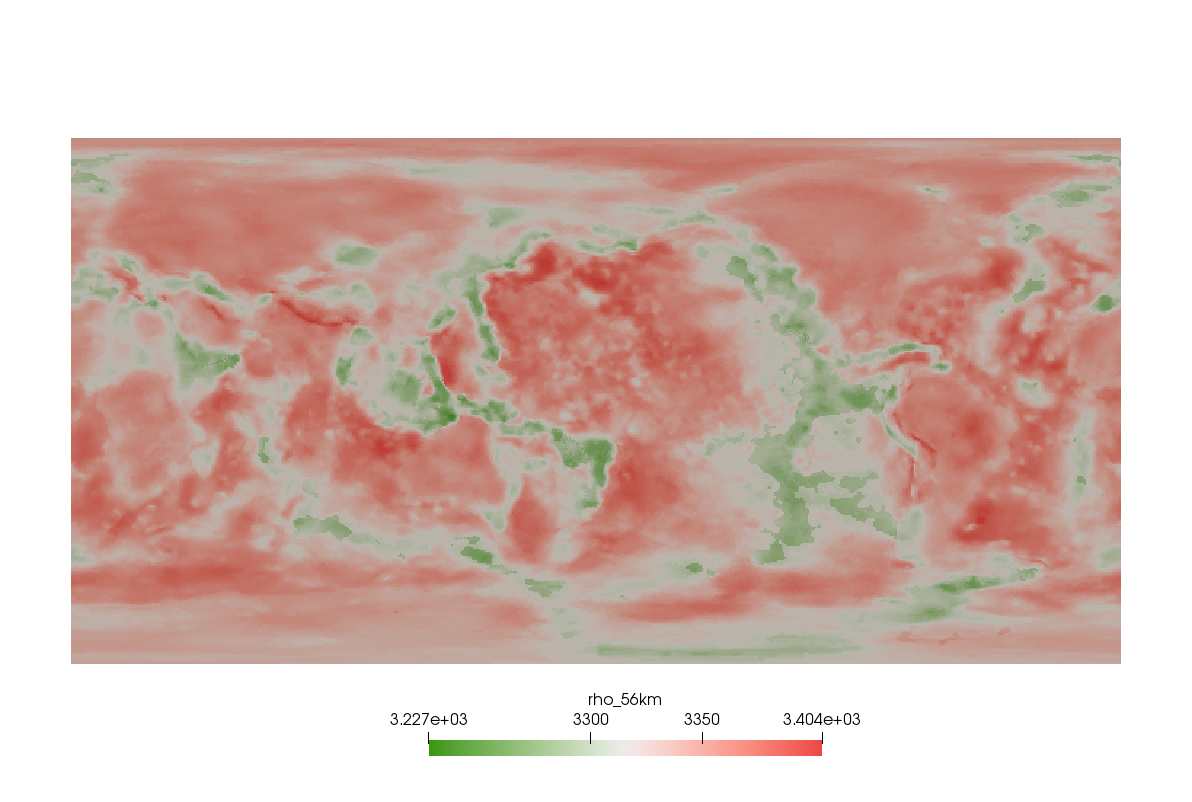
\includegraphics[width=8cm]{python_codes/fieldstone_99/images/rho_56}
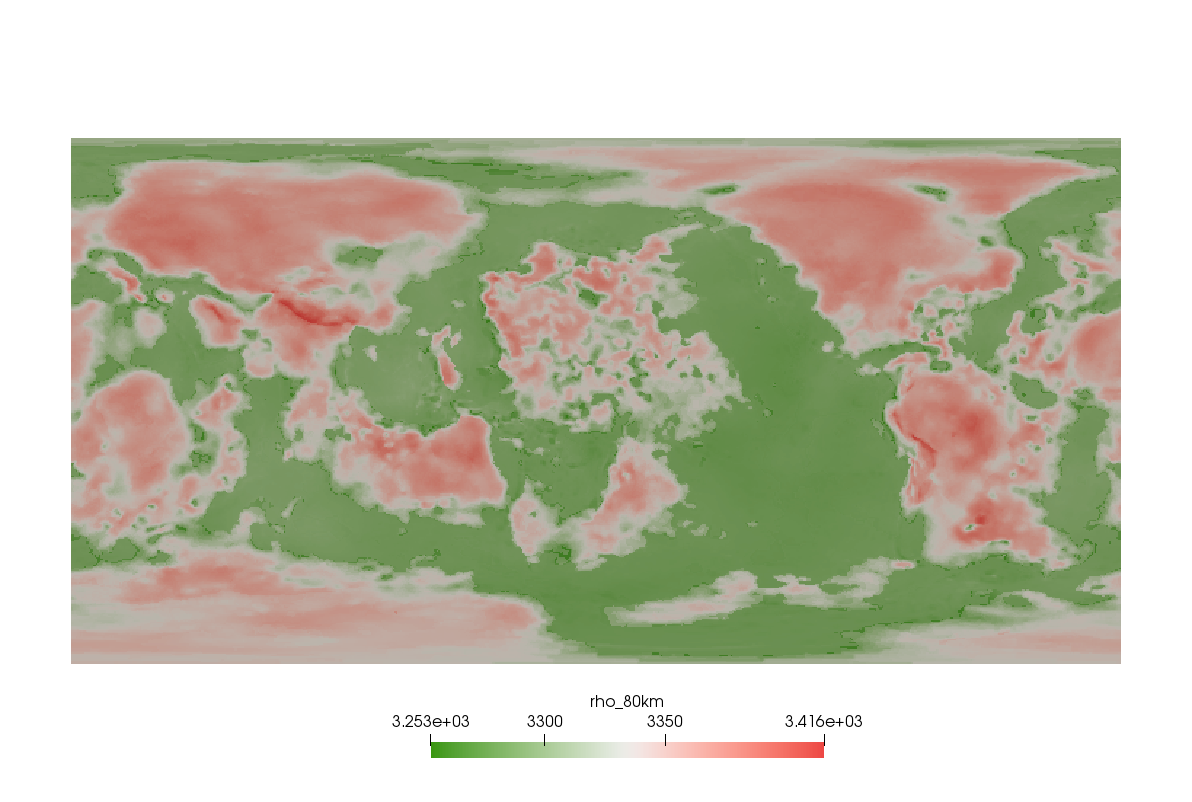
\includegraphics[width=8cm]{python_codes/fieldstone_99/images/rho_80}\\
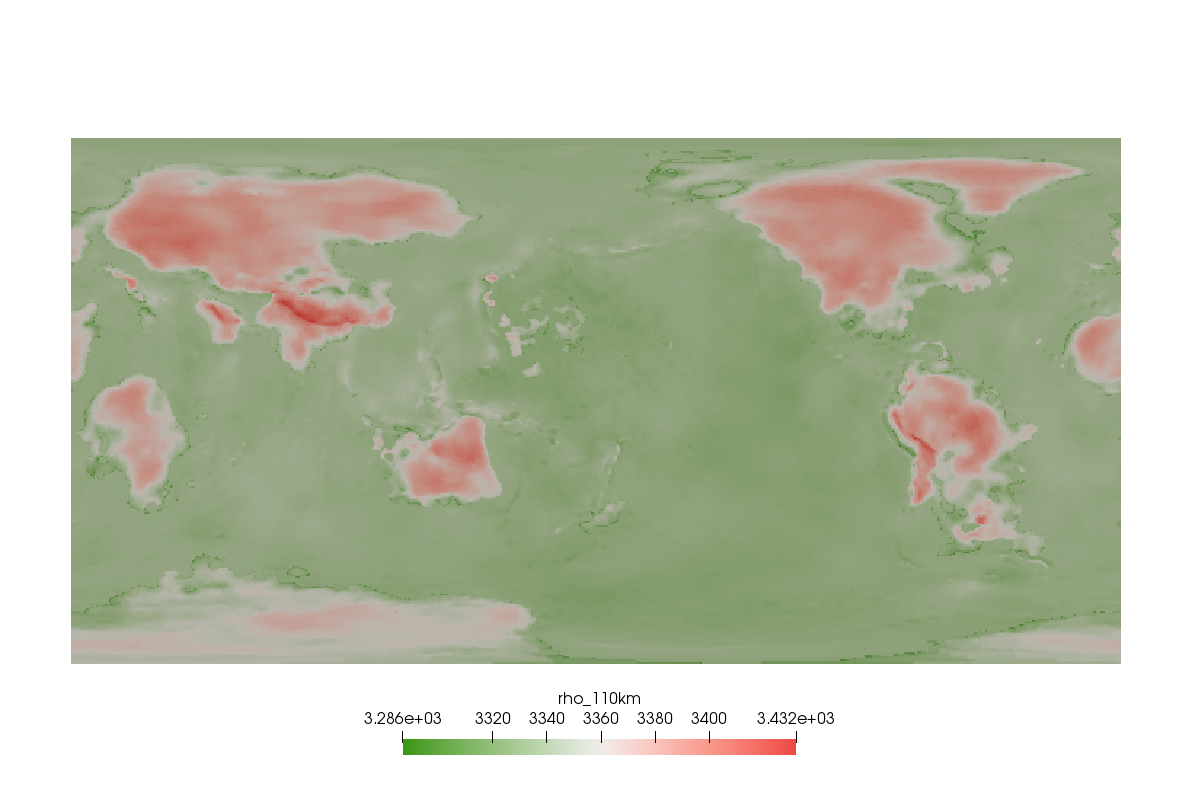
\includegraphics[width=8cm]{python_codes/fieldstone_99/images/rho_110}
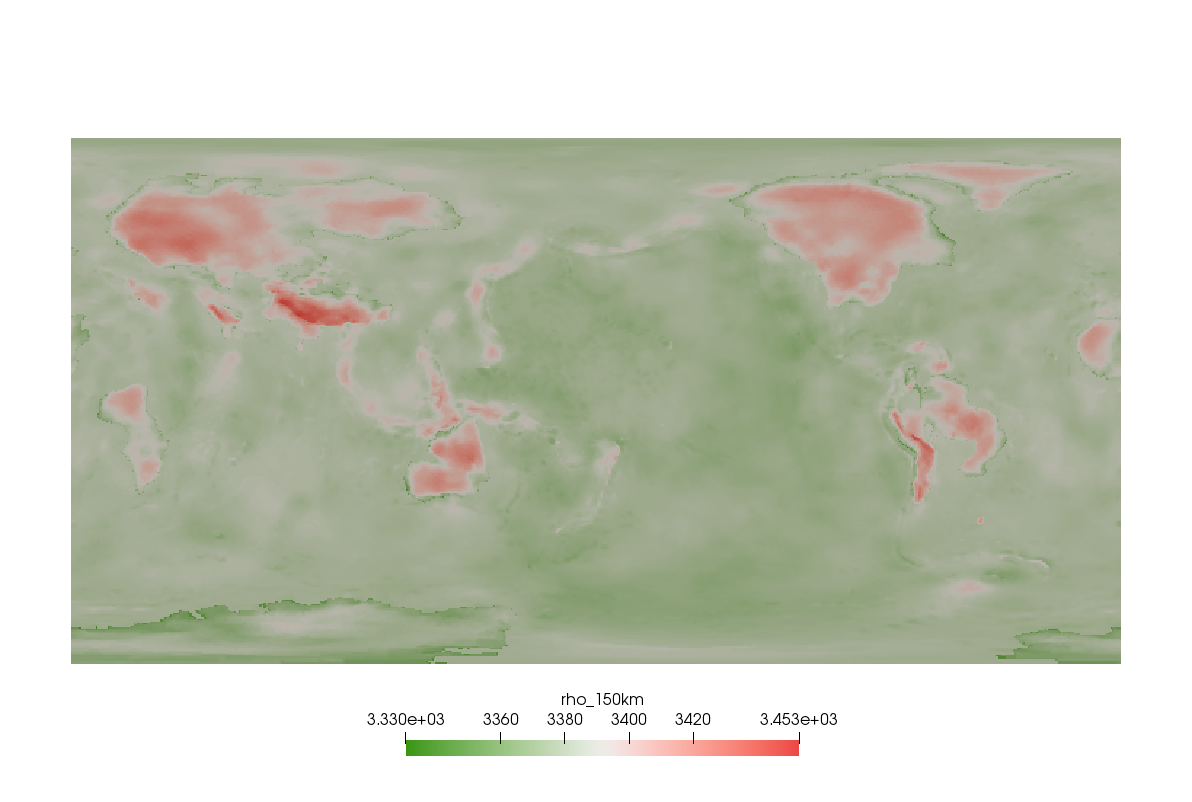
\includegraphics[width=8cm]{python_codes/fieldstone_99/images/rho_150}\\
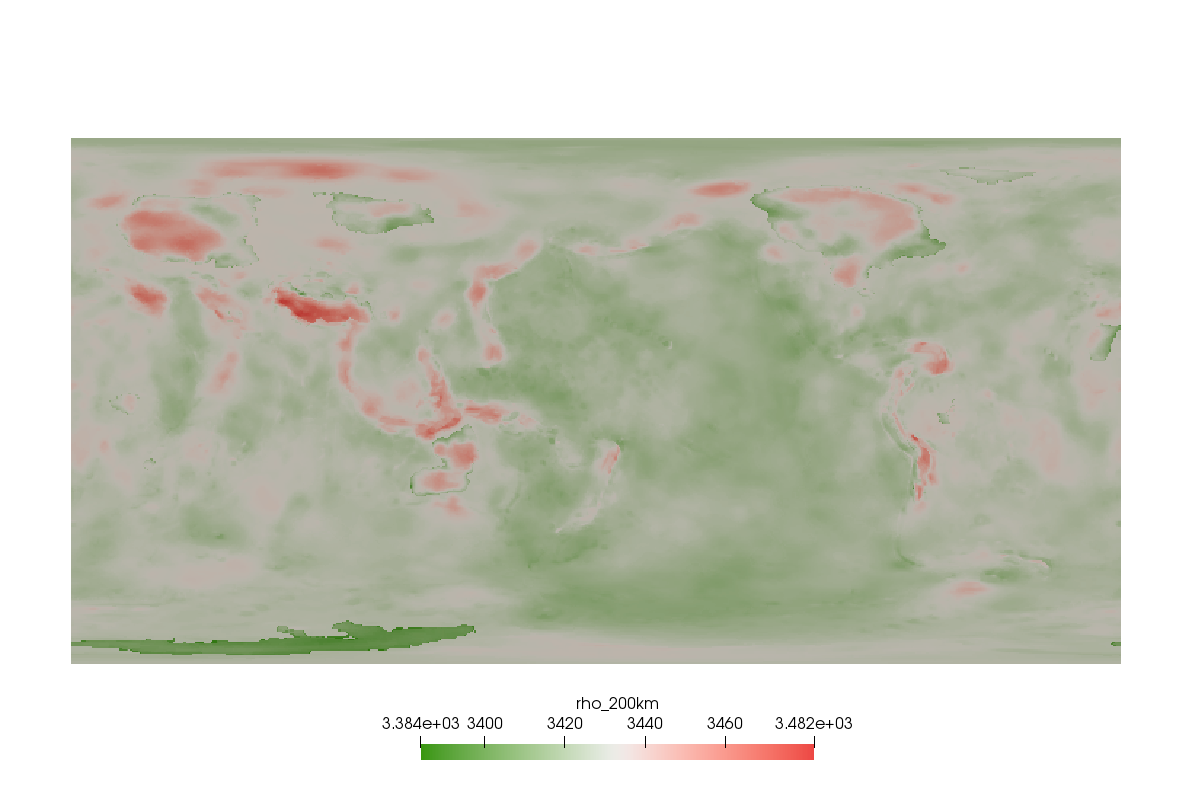
\includegraphics[width=8cm]{python_codes/fieldstone_99/images/rho_200}
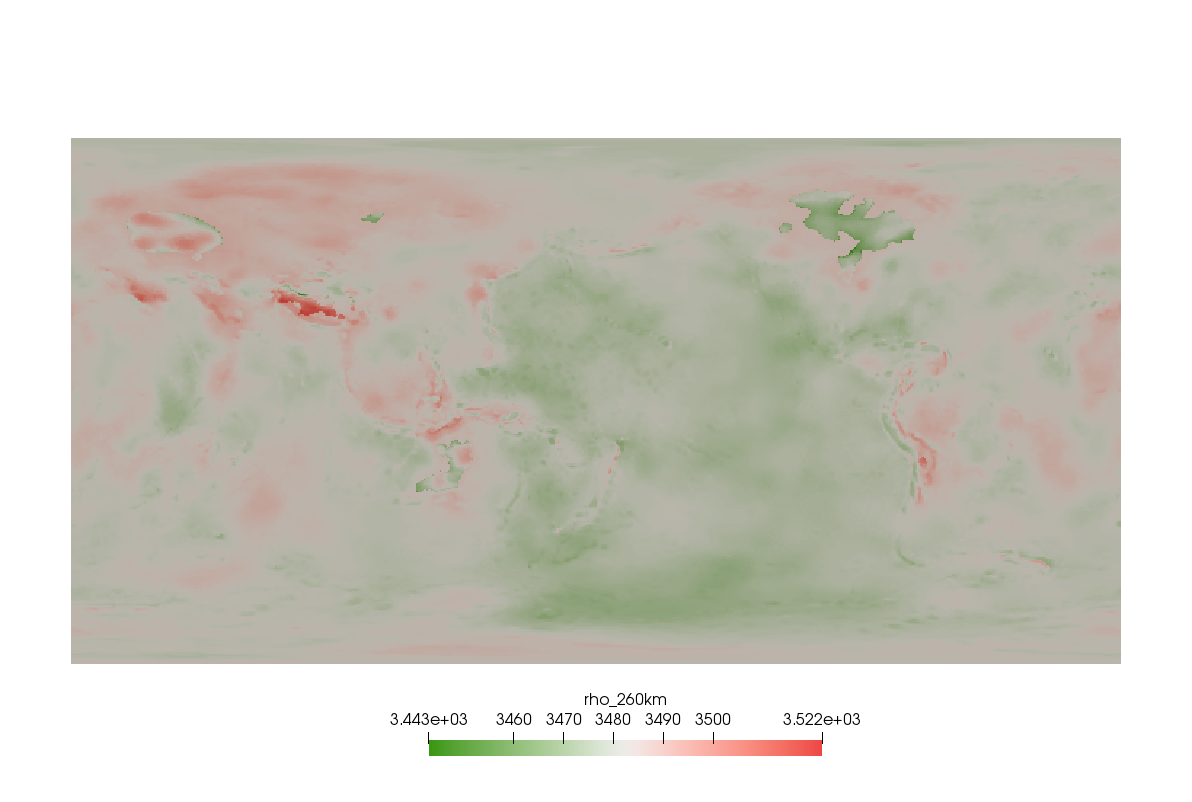
\includegraphics[width=8cm]{python_codes/fieldstone_99/images/rho_260}\\
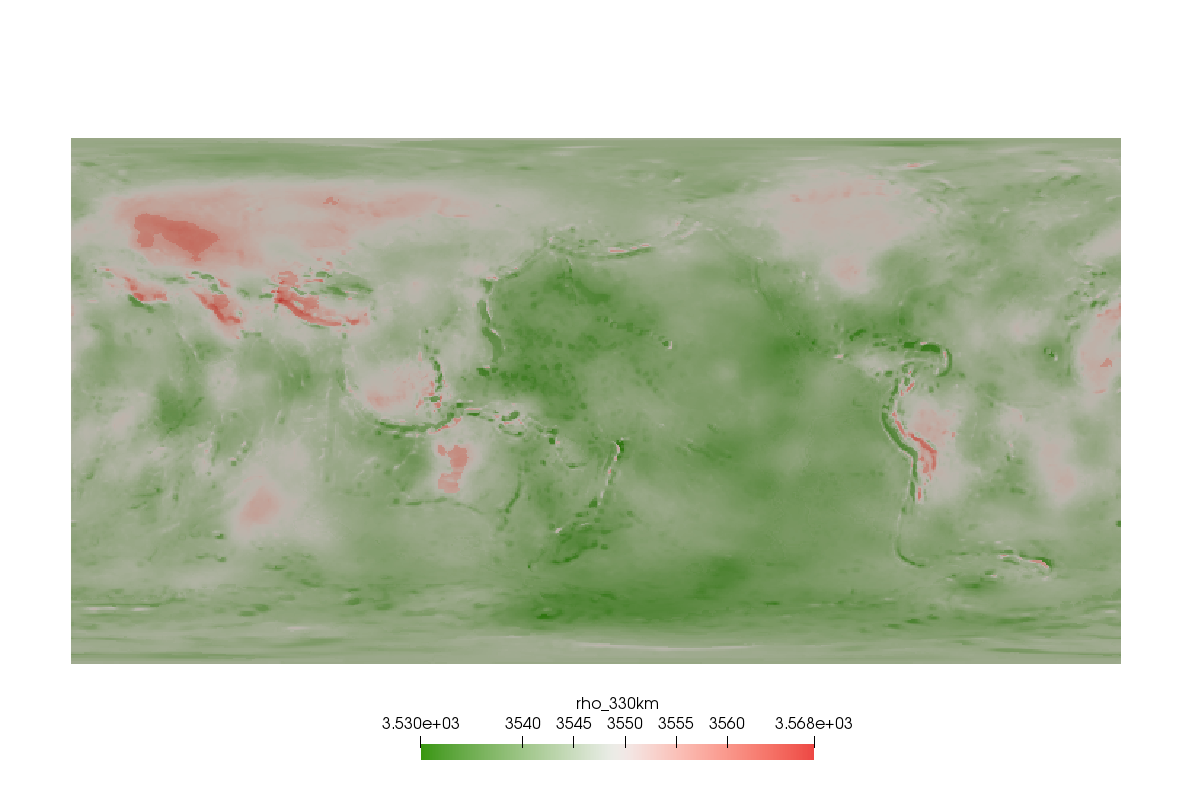
\includegraphics[width=8cm]{python_codes/fieldstone_99/images/rho_330}
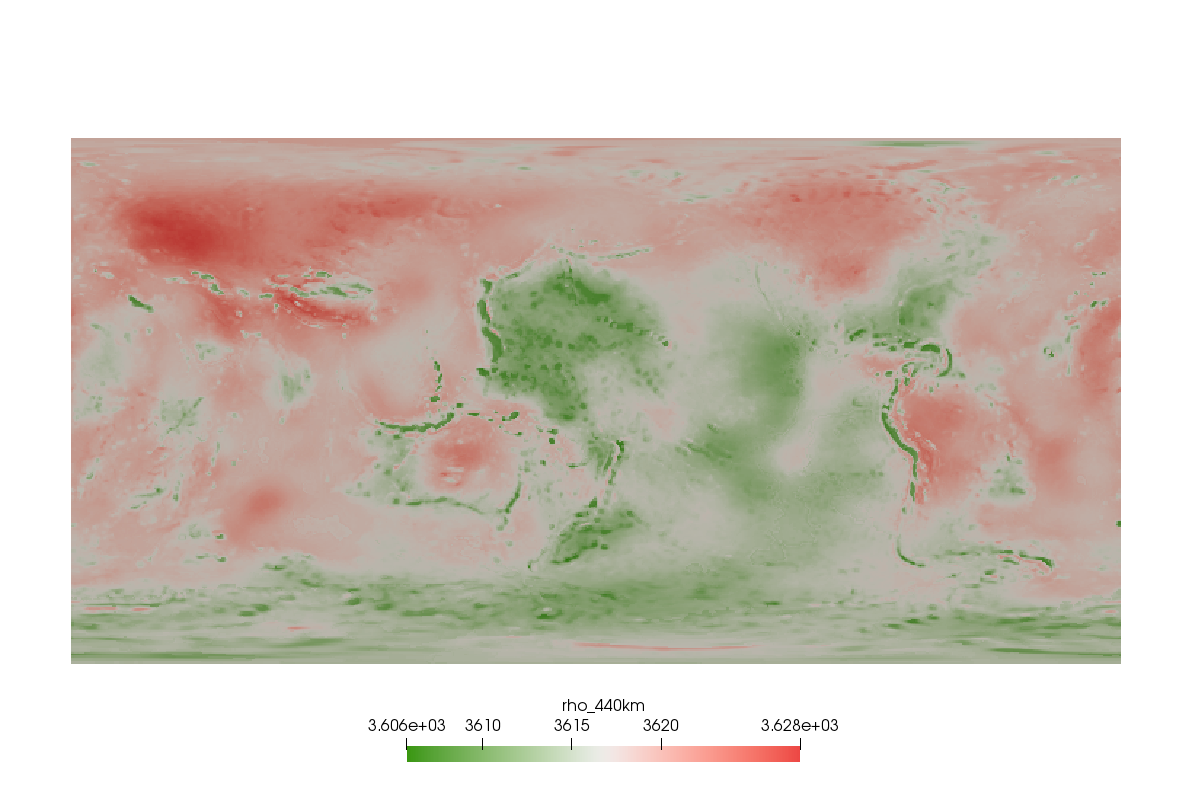
\includegraphics[width=8cm]{python_codes/fieldstone_99/images/rho_400}\\
{\captionfont Density values at depths 20, 36, 56, 80, 110, 150, 200, 260, 330, 400km.}
\end{center}


